\documentclass[12pt]{article}
\usepackage[danish]{babel}
\usepackage{amsfonts, amssymb, mathtools, amsthm, amsmath}
\usepackage{graphicx, pgfplots}
\usepackage{url}
\usepackage[dvipsnames]{xcolor}
\usepackage{sagetex}
\usepackage{lastpage}

%loaded last
\usepackage[hidelinks]{hyperref}

\usepackage{siunitx}
  \sisetup{exponent-product = \cdot,
    output-decimal-marker = {,}}

%Giles Castelles incfig
\usepackage{import}
\usepackage{xifthen}
\usepackage{pdfpages}
\usepackage{transparent}

\newcommand{\incfig}[2][1]{%
  \def\svgwidth{#1\columnwidth}
  \import{../figures/}{#2.pdf_tex}
}

\setlength{\parindent}{0in}
\setlength{\oddsidemargin}{0in}
\setlength{\textwidth}{6.5in}
\setlength{\textheight}{8.8in}
\setlength{\topmargin}{0in}
\setlength{\headheight}{18pt}

\usepackage{fancyhdr}
\pagestyle{fancy}

\fancyhead{}
\fancyfoot{}
\fancyfoot[R]{\thepage}
\fancyhead[C]{\leftmark}

\pgfplotsset{compat=newest}

\pgfplotsset{every axis/.append style={
  axis x line=middle,    % put the x axis in the middle
  axis y line=middle,    % put the y axis in the middle
  axis line style={<->,color=black}, % arrows on the axis
}}

\usepackage{thmtools}
\usepackage{tcolorbox}
  \tcbuselibrary{skins, breakable}
  \tcbset{
    space to upper=1em,
    space to lower=1em,
  }

\theoremstyle{definition}

\newtcolorbox[auto counter]{definition}[1][]{%
  breakable,
  colframe=ForestGreen,  %frame color
  colback=ForestGreen!5, %background color
  colbacktitle=ForestGreen!25, %background color for title
  coltitle=ForestGreen!70!black,  %title color
  fonttitle=\bfseries\sffamily, %title font
  left=1em,              %space on left side in box,
  enhanced,              %more options
  frame hidden,          %hide frame
  borderline west={2pt}{0pt}{ForestGreen},  %display left line
  title=Definition \thetcbcounter: #1,
}

\newtcolorbox{greenline}{%
  breakable,
  colframe=ForestGreen,  %frame color
  colback=white,          %remove background color
  left=1em,              %space on left side in box
  enhanced,              %more options
  frame hidden,          %hide frame
  borderline west={2pt}{0pt}{ForestGreen},  %display left line
}

\newtcolorbox[auto counter, number within=section]{eks}[1][]{%
  brekable,
  colframe=NavyBlue,  %frame color
  colback=NavyBlue!5, %background color
  colbacktitle=NavyBlue!25,    %background color for title
  coltitle=NavyBlue!70!black,  %title color
  fonttitle=\bfseries\sffamily, %title font
  left=1em,            %space on left side in box,
  enhanced,            %more options
  frame hidden,        %hide frame
  borderline west={2pt}{0pt}{NavyBlue},  %display left line
  title=Eksempel \thetcbcounter: #1
}

\newtcolorbox{blueline}{%
  breakable,
  colframe=NavyBlue,     %frame color
  colback=white,         %remove background
  left=1em,              %space on left side in box,
  enhanced,              %more options
  frame hidden,          %hide frame
  borderline west={2pt}{0pt}{NavyBlue},  %display left line
}

\newtcolorbox{teo}[1][]{%
  breakable,
  colframe=RawSienna,  %frame color
  colback=RawSienna!5, %background color
  colbacktitle=RawSienna!25,    %background color for title
  coltitle=RawSienna!70!black,  %title color
  fonttitle=\bfseries\sffamily, %title font
  left=1em,              %space on left side in box,
  enhanced,              %more options
  frame hidden,          %hide frame
  borderline west={2pt}{0pt}{RawSienna},  %display left line
  title=Teori: #1,
}

\newtcolorbox[auto counter, number within=section]{sæt}[1][]{%
  breakable,
  colframe=RawSienna,  %frame color
  colback=RawSienna!5, %background color
  colbacktitle=RawSienna!25,    %background color for title
  coltitle=RawSienna!70!black,  %title color
  fonttitle=\bfseries\sffamily, %title font
  left=1em,              %space on left side in box,
  enhanced,              %more options
  frame hidden,          %hide frame
  borderline west={2pt}{0pt}{RawSienna},  %display left line
  title=Sætning \thetcbcounter: #1,
  before lower={\textbf{Bevis:}\par\vspace{0.5em}},
  colbacklower=RawSienna!25,
}

\newtcolorbox{redline}{%
  breakable,
  colframe=RawSienna,  %frame color
  colback=white,       %Remove background color
  left=1em,            %space on left side in box,
  enhanced,            %more options
  frame hidden,        %hide frame
  borderline west={2pt}{0pt}{RawSienna},  %display left line
}

\newtcolorbox{for}[1][]{%
  breakable,
  colframe=NavyBlue,  %frame color
  colback=NavyBlue!5, %background color
  colbacktitle=NavyBlue!25,    %background color for title
  coltitle=NavyBlue!70!black,  %title color
  fonttitle=\bfseries\sffamily, %title font
  left=1em,              %space on left side in box,
  enhanced,              %more options
  frame hidden,          %hide frame
  borderline west={2pt}{0pt}{NavyBlue},  %display left line
  title=Forklaring #1,
}

\newtcolorbox{bem}{%
  breakable,
  colframe=NavyBlue,  %frame color
  colback=NavyBlue!5, %background color
  colbacktitle=NavyBlue!25,    %background color for title
  coltitle=NavyBlue!70!black,  %title color
  fonttitle=\bfseries\sffamily, %title font
  left=1em,              %space on left side in box,
  enhanced,              %more options
  frame hidden,          %hide frame
  borderline west={2pt}{0pt}{NavyBlue},  %display left line
  title=Bemærkning:,
}

\makeatother
\def\@lecture{}%
\newcommand{\lecture}[3]{
  \ifthenelse{\isempty{#3}}{%
    \def\@lecture{Lecture #1}%
  }{%
    \def\@lecture{Lecture #1: #3}%
  }%
  \subsection*{\makebox[\textwidth][l]{\@lecture \hfill \normalfont\small\textsf{#2}}}
}

\makeatletter

\newcommand{\opgave}[1]{%
 \def\@opgave{#1}%
 \subsection*{Opgave #1}
}

\makeatother

%Format lim the same way in intext and in display
\let\svlim\lim\def\lim{\svlim\limits}

% horizontal rule
\newcommand\hr{
\noindent\rule[0.5ex]{\linewidth}{0.5pt}
}

\title{Eksamen i: Fysik og Mekanik}
\author{Noah Rahbek Bigum Hansen}
\date{20. december 2023 (15. December 2024)}

\begin{document}

\maketitle

\section*{1.}
\begin{figure} [ht]
  \centering
  \caption{}
  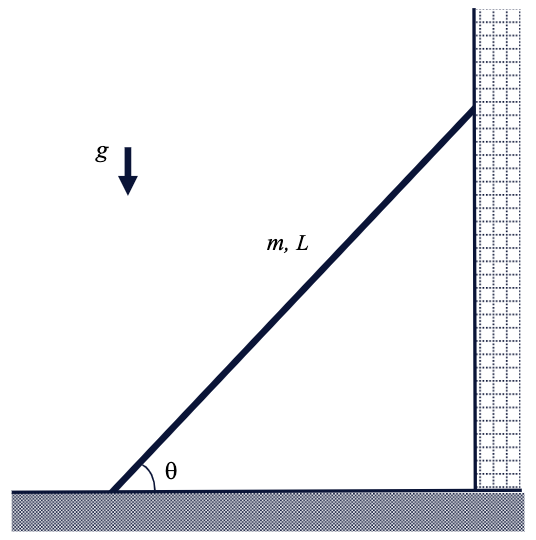
\includegraphics[width=0.5\linewidth]{../figures/E4_1.png}
  \label{fig:E4_1}
\end{figure}

Toppen af en stige med længden $L$ og massen $m$ hviler op ad en fuldstændig glat væg, medens foden af stigen hviler på en vandret asfalteret flade (\textbf{\autoref{fig:E4_1}}). Lad $\mu_s$ være den statiske friktionskoefficient  mellem  asfalt  og  stige,  og  lad  $g$ være  tyngdeaccelerationen.  Bestem  den  mindste  mulige vinkel $\theta$ mellem stigen og vandret hvorved stigen ikke glider.
\bigbreak
Idet vi ønsker at finde den mindst mulige vinkel netop hvor der er statik, må det gælde at der er statik i scenariet. Vi har derfor at
\[ 
\sum F_{x} = 0; \qquad \sum F_{y} = 0; \qquad \sum\tau = 0
.\]
\begin{figure}[ht]
  \centering
  \incfig[0.35]{E4_5}
  \caption{Fritlegemediagram}
  \label{fig:E4_5}
\end{figure}
Dermed kan flg. sammenhænge opstilles
\begin{align*}
  f_s - R &= 0 & &\implies & f_s &= R \\
  N - F_g &= 0 & &\implies & N &= mg \\
  R L \sin\theta - mg \frac{L}{2} \cos \theta &= 0 & &\implies & R \sin\theta &= mg \frac{1}{2} \cos\theta \\
.\end{align*}
Vi får da at
\[ 
R \tan\theta = \frac{1}{2}mg \implies R = \frac{1}{2}mg \frac{1}{\tan \theta}
.\]
Dette kan vi nu indsætte i udtrykket for friktionskraften som
\begin{align*}
  f_s &\geq R \\
  mg \mu &\geq\frac{1}{2}mg \frac{1}{\tan\theta}\\
  \tan\theta &\geq  \frac{1}{2\mu} \\
  \theta &\geq \tan^{-1} \frac{1}{2\mu}
.\end{align*}


\section*{2.}
\begin{figure} [ht]
  \centering
  \caption{}
  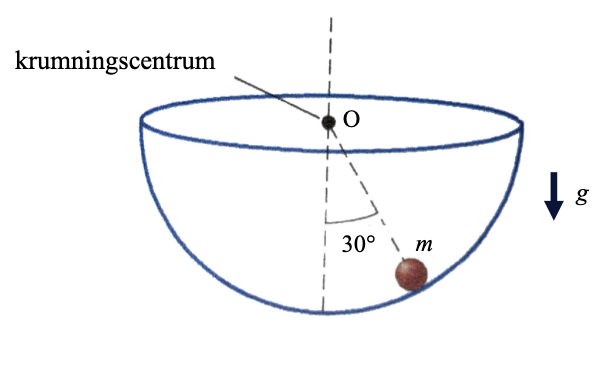
\includegraphics[width=0.5\linewidth]{../figures/E4_2.png}
  \label{fig:E4_2}
\end{figure}

En sfærisk perle med massen $m$ ligger i en skål med form af en hemisfære (dvs. en halvkugle-formet skal), som vist i \textbf{\autoref{fig:E4_2}}. Perlen rulles lidt op ad skålens inderside, hvorefter den frigøres. Perlen ruller uden at glide. Perlens begyndelsesposition er således, at en imaginær linje tegnet fra dens centrum til skålens centrum $O$ (krumningscentrum; eng: center of curvature) danner en vinkel på \ang{30}  med lodret; se igen \textbf{\autoref{fig:E4_2}}. Perlens radius $r= \qty{10}{mm} $, medens skålens radius $R = \qty{100}{mm}$. Det kan antages at tyngdeaccelerationen $g = \qty{9,80}{m\per s^2} $. Bestem perlens vinkelhastighed $\omega$ omkring dens egen massemidtpunkt i det øjeblik den er i skålens bund.
\bigbreak
Idet det antages at der kan ses bort fra friktion er der mekanisk energibevarelse. Altså har vi at
\[
k_{0} + U_{0} = k_{1} + U_{1}
.\]
Idet perlen antages at have en hastighed $v_0 = 0$ idet den slippes og nulpunktet for højden $y = 0$ sættes til skålens bund reduceres det ovenstående til
\begin{equation} \label{eq:ekonsp}
  0 + U_{0} = k_{1} + 0 \implies U_0 = k_1
\end{equation}
Perlens starthøjde $y_0$ kan findes vha. trigonometri som
\begin{align*}
  y_0 = R - \cos \theta \cdot R = \qty{100}{mm} - \cos \ang{30} \cdot \qty{100}{mm} =  \qty{13,4}{mm} 
.\end{align*}
Jf. \autoref{eq:ekonsp} er perlens kinetiske energi på bunden af skålen
\begin{equation} \label{eq:kinp}
  k_1 = mgy_0 = m \cdot \qty{9,80}{\frac{m}{s^2}} \cdot \qty{13,4}{mm} = \qty{0,131}{\frac{m^2}{s^2}} m
\end{equation}
Den samlede kinetiske energi $k_1$ for perlen består både af et bidrag fra dens rotationelle kinetiske og fra dens translatoriske kinetiske energi. Altså
\[ 
k_1 = \frac{1}{2}mv_{cm}^2 + \frac{1}{2}I_{cm}\omega^2
.\]
Hastigheden af massemidtpunktet $v_{cm}$ for et objekt der ruller uden glidning er givet som
\[ 
v_{cm} = r\omega
.\]
Hvis udtrykket for hastigheden af massemidtpunktet $v_{cm}$ sættes ind i udtrykket for den samlede kinetiske energi $k_1$ fås at
\[ 
k_1 = \frac{1}{2}m r^2\omega^2 + \frac{1}{2}I_{cm}\omega^2
.\]
Inertimomentet for perlen omkring dens massemidtpunkt $I_{cm} = \frac{2}{5}mr^2$, idet denne kan modelleres som en solid kugle. Indsættes \label{eq:kinp} i det ovenstående fås at
\begin{align*}
  \qty{0,131}{\frac{m^2}{s^2}} m &= \frac{1}{2}m r^2 \omega^2 + \frac{1}{2}I_{cm}\omega^2 \\
  \qty{0,131}{\frac{m^2}{s^2}} m &= \frac{1}{2}m r^2 \omega^2 + \frac{1}{2} \cdot \frac{2}{5}mr^2 \omega^2 \\
  \qty{0,131}{\frac{m^2}{s^2}} &= \frac{7}{10} r^2 \omega^2 \\
  \omega^2 &= \frac{10}{7} \cdot \qty{0,131}{\frac{m^2}{s^2}} \frac{1}{r^2} \\
  \omega &= \sqrt{\frac{10}{7} \cdot \qty{0,131}{\frac{m^2}{s^2}} \cdot \frac{1}{(\qty{10}{mm})^2}} \\
  \omega &= \qty{43,3}{s^{-1}} 
.\end{align*}
Altså er perlens vinkelhastighed om sit eget massemidtpunkt i det den når bunden af skålen \underline{\underline{$\omega = \qty{43,3}{s^{-1}}$}}

\section*{3.}
\begin{figure} [ht]
  \centering
  \caption{}
  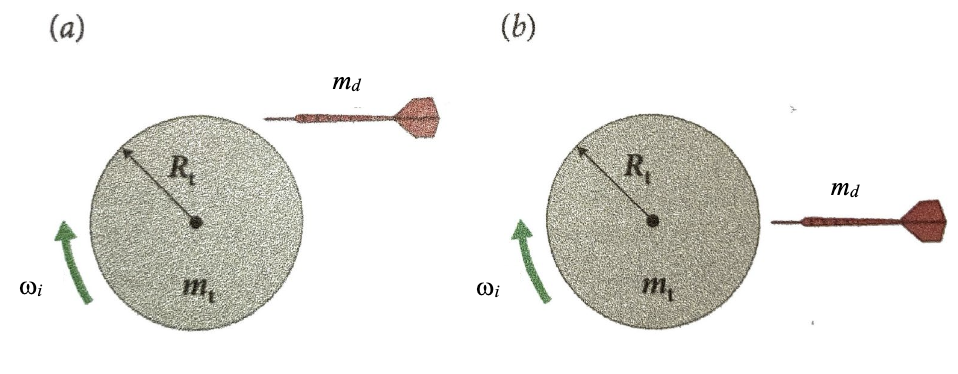
\includegraphics[width=0.5\linewidth]{../figures/E4_3.png}
  \label{fig:E4_3}
\end{figure}

En jævntyk skive (eng.: disk) med radius $R_t$ og masse $m_t$ roterer med uret, med vinkelhastigheden $\omega_i$ omkring en akse som går gennem skivens centrum og som er vinkelret på skivens plan. En dartpil med massen $m_d$ kastes ind mod skiven fra højre, som vist i \textbf{\autoref{fig:E4_3} (a,b)}. Dartpilen rammer skiven med hastigheden $v_d$ (mod venstre). Det kan antages at hele dartpilens masse er koncentreret i dens spids. Der kan ses bort fra tyngdeaccelerationen.


\subsection*{(a)}
Bestem den resulterende vinkelhastighed $\omega_f$ hvis dartpilen rammer tangentielt til skivens periferi, således at dartpilens spids borer sig ind i skivens yderkant, som indikeret i \textbf{\autoref{fig:E4_3} (a)}.
\bigbreak
Grundet konservation af impulsmoment har vi at
\[ 
L_0 = L_1 \implies -I_t \cdot \omega_i + R_t \cdot m_d \cdot v_d = (I_t + m_d \cdot R_t^2)\omega_f
.\]
Den resulterende vinkelhastighed $\omega_f$ kan da isoleres som
\begin{align*}
  \omega_f &= \frac{-I_t \cdot \omega_i + R_t \cdot m_d \cdot v_d}{I_t + m_d \cdot R_t^2} \\
  &= \frac{-\frac{1}{2}m_t R_t^2 \cdot \omega_i + R_t \cdot m_d \cdot v_d}{\frac{1}{2}m_t R_t^2 + m_d \cdot R_t^2} \\
  &= \frac{m_d \cdot v_d \cdot \frac{1}{R_t} - \frac{1}{2}m_t \cdot \omega_i}{\frac{1}{2}m_t + m_d}
.\end{align*}
Altså er den resulterende vinkelhastighed, hvis dartpilen rammer som vist på \textbf{\autoref{fig:E4_3} (a)} \underline{\underline{$\omega_f = \frac{m_dv_d \frac{1}{R_t} - \frac{1}{2}m_t\omega_i}{\frac{1}{2}m_t + m_d}$}}.


\subsection*{(b)}
Bestem den resulterende vinkelhastighed $\omega_f$ hvis dartpilens spids i stedet rammer skiven -- og borer sig ind i denne -- langs en normal, dvs. langs en linje som går gennem skivens centrum som indikeret i \textbf{\autoref{fig:E4_3} (b)}.
\bigbreak
I dette tilfælde har dartpilen ikke nogen ``kraftarm'' og den har derfor intet impulsmoment. Vi får derfor fra impulsmomentkonservation at
\[ 
L_0 = L_1 \implies -I_t \cdot \omega_i = \left( I_t + m_d \cdot R_t^2 \right)\omega_f
.\]
I dette udtryk kan vi igen isolere den resulterende vinkelhastighed $\omega_f$ som
\begin{align*}
  \omega_f &= \frac{-\frac{1}{2}m_t R_t^2 \cdot \omega_i}{\frac{1}{2}m_t R_t^2 + m_d R_t^2} \\
  &= \frac{-\frac{1}{2}m_t\omega_i}{\frac{1}{2}m_t + m_d}
.\end{align*}
Dermed har vi for tilfældet, hvor dartpilen rammer skiven langs en normal (\textbf{\autoref{fig:E4_3} (b)}) at den resulterende vinkelhastighed \underline{\underline{$\omega_f = -\omega_i \frac{\frac{1}{2}m_t}{\frac{1}{2}m_t + m_d}$}}

\section*{4.}
\begin{figure} [ht]
  \centering
  \caption{}
  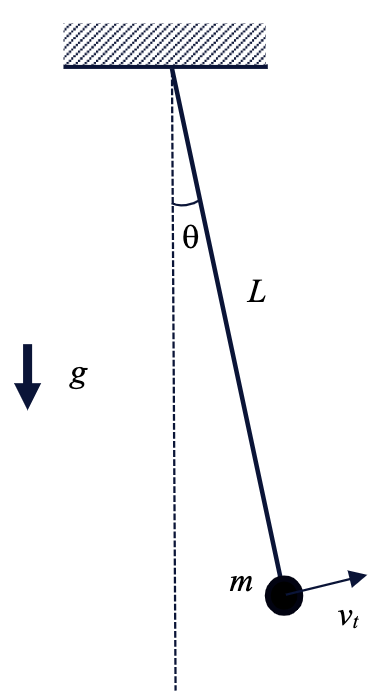
\includegraphics[width=0.3\linewidth]{../figures/E4_4.png}
  \label{fig:E4_4}
\end{figure}

Et simpelt (matematisk) pendul, bestående af en tynd snor med længden $L = \qty{0,30}{m}$ og en kugle med massen $m = \qty{0,30}{kg}$, udfører harmoniske svingninger omkring ligevægtspositionen $\theta = 0$, se \textbf{\autoref{fig:E4_4}}. Når massen $m$ passerer det laveste punkt (ligevægtspositionen $\theta = 0$) har $m$ den tangentielle (og horisontale) hastighed $|v_t| = \qty{0,25}{m \per s}$. Lad $g$ betegne tyngdeaccelerationen ($g = \qty{9,80}{m \per s^2}$).

\subsection*{(a)}
Bestem den maksimale vinkeldrejning (vinkelforskydning) $\theta_{max}$, bort fra den vertikale ligevægtsposition, som pendulet opnår.
\bigbreak
Idet det antages at pendulet er perfekt og derfor ikke har nogen friktion må der være energibevarelse. Altså gælder at den kinetiske energi idet pendulet passerer bunden $k_0$ må blive omdannet fuldstændig til en potentiel energi $U_1$ før pendulet stopper med at bevæge sig opad. Altså kan højden $y$ til pendulets maksimalforskydning findes som
\begin{align*}
  mgy_{maks} &= \frac{1}{2}mv^2 \\
  y_{maks} &= \frac{1}{2} \frac{v^2}{g} \\
  &= \frac{1}{2} \cdot \frac{\left( \qty{0,25}{\frac{m}{s}}  \right)^2}{\qty{9,80}{\frac{m}{s}}} \\
  &= \qty{0,0031887755}{m} 
.\end{align*}
(\textit{Bemærk:} Årsagen til at der er medtaget så mange decimaler som der er i udregningen ovenfor er for at undgå afrundingsfejl senere -- dette er specielt vigtigt her fordi vinklen bliver relativt lille).

Ved pendulets maksimale udstrækning vil den lodrette afstand til det punkt, hvor pendulet er fastgjort altså være $L - y_{maks}$. Vi kan dernæst finde den maksimale vinkeldrejning $\theta_{max}$ vha. trigonometri som
\[ 
\theta_{maks} = \cos^{-1} \frac{L- y_{maks}}{L} = \cos^{-1} \frac{\qty{0,30}{m} - \qty{0,0031887755}{m}}{\qty{0,30}{m}} = \ang{8,4} 
.\]
Altså er den maksimale vinkeldrejning \underline{\underline{$\theta_{maks} = \ang{8,4} $}}




\subsection*{(b)}
Bestem den tangentielle hastighed $v_t$ når vinkeldrejningen $\theta = \theta_{max} / 2$
\bigbreak
Når vinkeldrejningen $\theta = \theta_{maks} / 2 = \ang{4,2}$ har pendulet en højde på
\[ 
h = L - \cos \theta \cdot L = \qty{0,30}{m}  - \cos \ang{4,2} \cdot \qty{0,30}{m} = \qty{0,000805656832662982}{m} 
.\]
Vi kan nu igen benytte konservation af mekanisk energi som
\[ 
k_0 + U_0 = k_1 + U_1
.\]
Her sættes nulpunktet til pendulets bund, således at leddet for den initiale potentielle energi udgår og slutpunktet sættes til punktet, hvor vinkeldrejningen $\theta = \theta_{max} / 2$. Således fås
\begin{align*}
  \frac{1}{2}m \cdot v_i^2 &= \frac{1}{2}m \cdot v_f^2 + mgh \\
  v_f^2 &= v_i^2 - gh \\
  v_f &= \sqrt{v_i^2 - gh} \\
  &= \sqrt{\left(\qty{0,25}{\frac{m}{s}}\right)^2 - \cdot \qty{9,8}{\frac{m}{s^2}} \cdot \qty{0.000805656832662982}{m}} \\
  &= \qty{0,234}{\frac{m}{s}}  
.\end{align*}
Altså er hastigheden af pendulet \underline{\underline{$\qty{0,234}{m \per s}$}}til vinklen $\theta = \theta_{max} / 2$.

\end{document}
